
\section{Conclusiones}

\subsection{PageRank}
Este algoritmo resultó bastante sencillo de implementar, una gran parte del mismo fue la implementación de la matriz esparsa para mejorar tanto la performance espacial como la temporal en el cálculo del método de la potencia. \\
En cuanto a tiempos es bastante estable y podemos deducir bajo las pruebas realizadas que debería seguir siendo así para grafos aún más grandes. A contrapartida, la calidad si bien es muy buena para c$=$0.15, lo que confirma el comentario en el paper original, notamos que hay un trabajo grande por encima en los buscadores reales pero es un muy buen punto de partida. Nos referimos a posicionamiento por publicidad, eliminación de SPAM, etc.

\subsection{HITS}

Una parte importante sobre este algoritmo es que tarda mucho para nodos grandes, sin embargo no debemos olvidar que en su paper$[2]$ Kleinberg habla de que este algoritmo debe ser aplicado no sobre toda la red sin sobre un subconjunto de la misma ($\textit{root set}$) obtenido de una busqueda incial. Por lo tanto si acotamos el análisis a los grafos mas acotados podemos ver que el tiempo de computo es aceptable y hasta muy parecido al de page rank. 
Si el algoritmo aplicado en la red fuese HITS lo recomendable al cliente sería que negocie con los principales HUBS para que apunten a su sitio. Logrando así rankear mejor en la sección de Autoridades sobre el tema. 
No le recomendaríamos que negocie con las páginas autoridades ya que dificilmente estas accediesen debido a que de esta manera se estarían restando puntos en el ranking de autoridades.\\
Por ejemplo en el caso de death penalty habría que negociar con alguno de los 3 principales HUBS: clarkprosecutor.org, faculty.etsu.edu o coramnobis.com. Teniendo en cuenta el costo de cada uno, ya que si el primero costase el doble 
o mas que el segundo tal vez convendría más negociar con el segundo y tercero.

\subsection{INDEG}
Este algoritmo es bastante simple y en una red chica y confiable puede llegar a valer. Es muy rápido y en caso de necesitar algún dato rápido, es muy fácil de implementar. Igualmente tiene mucho peso la confiabilidad, ya que es muy simple de crecer tu puntaje, simplemente comprando un lugar mínimo en la mayor cantidad de páginas posibles.\\
En cuanto a estrategia para mejorar el posicionamiento de tu sitio bajo este algoritmo es conseguir la mayor cantidad de páginas para que te apunten sin importar qué calidad de sitio.

%  \begin{figure}[!htb]
% \begin{center}
%     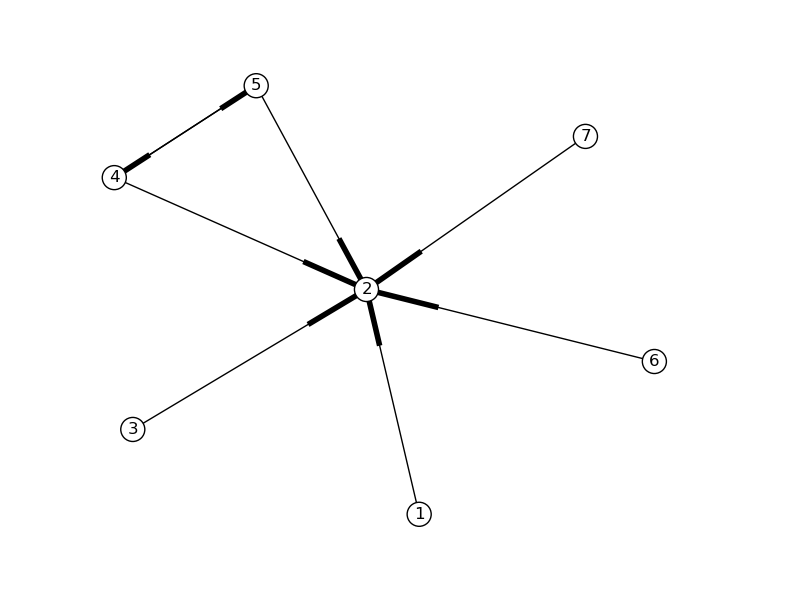
\includegraphics[scale=0.5]{imagenes/test4.png}
%     \caption{Red de 7 nodos}
%     \end{center}
% \end{figure}

\subsection{Mejor estrategia para comprar links}
\subsubsection{PageRank}

En esta sección intentaremos analizar distintas instancias de una red para analizar cual es la estrategia más conveniente a la hora de comprar links para aumentar el PageRank 
Como explicamos anteriormente, para el algoritmo de PageRank es más importante la calidad del sitio de entrada antes que la cantidad. Por lo tanto para encontrar la mejor estrategia intentaremos ver como se comporta la red para un sitio en especial variando los links que lo apunta. Para esto nos quedaremos con los primeros sitios de mayor pagerank de la red original y entre esos iremos variando entre diferentes conjuntos que tengan diferentes cantidades de links de salida y observando en que posición final queda nuestro sitio \\
En este caso analiceramos como se posiciona el sitio de los Wachiturros (www.wachiturros.com) bajo diferentes combinaciones de sitios que lo linkean en el set de datos \textbf{Death Penalty} que venimos utilizando en las anteriores secciones.\\

Ahora hagamos las siguientes prueba, apuntemos a los Wachiturros por distintas combinaciones de las primeras 10 posiciones que muestran los resultados del set de datos y analicemos en la posición que queda el sitio en cada caso:

   $$ 
\begin{bmatrix}
              		&      Ranking \\
 10\ sitios 		&   	12         \\
 5\ primeros   		&     	27   \\
 5\ segundos   		&      	65 	\\
 Mejor\ sitio   		&        122    \\
 5\ menos\ salidas  	&        16     \\
 4\ menos\ salidas  	&        19  \\
 3\ menos\ salidas   	&     	34 \\
\end{bmatrix} 
$$

Como se puede ver por los resultados, 




